%%%%%%%%%%%%%%%%%%%%%%%%%%%%%%%%%%%%%%%%%%%%%%%%%%%%%%%%%%%%%%%%%%%%%%%%%%%%%%%
% intro.tex: Introduction to the thesis
%%%%%%%%%%%%%%%%%%%%%%%%%%%%%%%%%%%%%%%%%%%%%%%%%%%%%%%%%%%%%%%%%%%%%%%%%%%%%%%%
\chapter{Introduction} \label{chap:intro}
\label{intro_chapter}
%%%%%%%%%%%%%%%%%%%%%%%%%%%%%%%%%%%%%%%%%%%%%%%%%%%%%%%%%%%%%%%%%%%%%%%%%%%%%%%%
\section{Decompositions}
Suppose you have $n$ translucent sheets of tracing paper with some points drawn on all $n$ sheets of paper in the same set arrangement. Now, draw lines connecting points on each sheet of paper, so that no line appears on two distinct sheets of paper.

A graph $K$ is depicted when all $n$ sheets of tracing paper are aligned and stacked on top of each other with some light source present. Call the graph depicted on the $i$th sheet of paper $G_{i}$ for $i=1,\hdots,n$. The stacking of these sheets of paper depicts the edge-disjoint union $G_{1}\cup \cdots \cup G_{n}=K$, and this collection of papers depicts the set $\{G_{1},\hdots,G_{n}\}$ which we call a \textit{graph decomposition} of $K$. This is defined formally below.

\begin{definition}[Graph Decomposition]
Let $K$ be a simple graph. We call a collection $\{G_{1},\hdots,G_{n}\}$ of pairwise edge-disjoint subgraphs $G_{1},\hdots,G_{n}\subseteq K$ of $K$ a \textit{decomposition} of $K$ if their union equals $K$.
\end{definition}
\begin{figure}[H]
  \begin{center}
      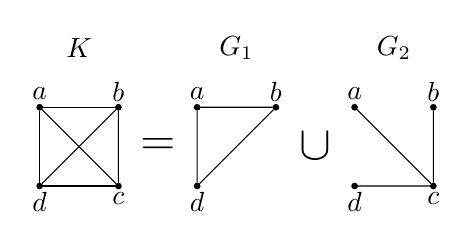
\begin{tikzpicture}[every node/.style={draw, circle, fill=black, minimum size=2pt, inner sep=0pt}]
          % First Graph
          \node (T)[draw=none, fill=none] at (0.5,0.75) {$K$};
          \node (0) at (0, 0)[label=above:$a$]  {};
          \node (1) at (1, 0)[label=above:$b$]  {};
          \node (2) at (1, -1)[label=below:$c$] {};
          \node (3) at (0, -1)[label=below:$d$] {};

          \draw (2) -- (3) -- (0) -- (1);
          \draw (0) -- (2) -- (1) -- (3);
          % "=" symbol
          \node[draw=none, fill=none] at (1.5, -0.5) {\LARGE $=$};

          % Second graph
          \begin{scope}[xshift=2cm]
            \node (T)[draw=none, fill=none] at (0.5,0.75) {$G_{1}$};
            \node (0) at (0, 0)[label=above:$a$]  {};
            \node (1) at (1, 0)[label=above:$b$]  {};
            \node (3) at (0, -1)[label=below:$d$] {};

              \draw (0) -- (1) -- (3) -- (0);
          \end{scope}
          
          % "\cup" symbol
          \node[draw=none, fill=none] at (3.5, -0.5) {\LARGE $\cup$};
          
          \begin{scope}[xshift=4cm]
            \node (T)[draw=none, fill=none] at (0.5,0.75) {$G_{2}$};
            \node (0) at (0, 0)[label=above:$a$]  {};
            \node (1) at (1, 0)[label=above:$b$]  {};
            \node (2) at (1, -1)[label=below:$c$] {};
            \node (3) at (0, -1)[label=below:$d$] {};
              
            \draw (3) -- (2) -- (0) -- (2) -- (1);
          \end{scope}
      \end{tikzpicture}
  \end{center}
  \caption{$\{G_{1},G_{2}\}$ is a decomposition of $K_{4}$}
  \label{fig:simpledecompex}
\end{figure}

\newpage Graph decompositions are an important topic in combinatorics, graph theory, and design theory, with origins dating back to the 1800s. Notably, in 1850 Reverend Thomas Kirkman, a full-time clergyman and legendary mathematician, posed an important problem in \textit{The Lady's and Gentleman's Diary}~\cite{Kirkman1850} now known as \textit{the school girl problem}. It goes

\begin{center}
\begin{minipage}{0.7\textwidth}
  \centering\itshape
  Fifteen young ladies in a school walk out three abreast for seven days in succession: it is required to arrange them daily so that no two shall walk twice abreast.
\end{minipage}
\end{center}

The problem asks if we can form five distinct rows of three school girls on each day of the week so that no two school girls walk in the same row more than once in a week. This is equivalent to finding a decomposition of $K_{15}$ whose members are all triangles; whose members are isomorphic to $C_{3}$ or $K_{3}$. Both Kirkman and Arthur Cayley independently solved the the schoolgirl problem and published their solutions in the 1851 edition of \textit{The Lady's and Gentleman's Diary}~\cite{Kirkman1851}. Kirkman's solution is provided below.

  \vspace{1em}
  \itshape
  \noindent Denoting the ladies by $a_1, a_2, a_3$; $b_1, b_2, b_3$; $c_1, c_2, c_3$; $d_1, d_2, d_3$; $e_1, e_2, e_3$, the following arrangement will be found to answer the question:
\[
\renewcommand{\arraystretch}{0.7}
\begin{array}{
  @{}c@{\hskip 2pt}c@{\hskip 2pt}c
  |c@{\hskip 2pt}c@{\hskip 2pt}c
  |c@{\hskip 2pt}c@{\hskip 2pt}c
  |c@{\hskip 2pt}c@{\hskip 2pt}c
  |c@{\hskip 2pt}c@{\hskip 2pt}c
  |c@{\hskip 2pt}c@{\hskip 2pt}c
  |c@{\hskip 2pt}c@{\hskip 2pt}c@{}}
a_1 & a_2 & a_3 & a_1 & b_1 & c_1 & a_1 & d_1 & e_1 & a_1 & b_2 & d_2 & a_1 & c_2 & e_2 & a_1 & b_3 & e_3 & a_1 & c_3 & d_3 \\
b_1 & b_2 & b_3 & a_2 & b_2 & c_2 & a_2 & d_2 & e_2 & a_2 & b_3 & d_3 & a_2 & c_3 & e_3 & a_2 & b_1 & e_1 & a_2 & c_1 & d_1 \\
c_1 & c_2 & c_3 & a_3 & d_3 & e_3 & a_3 & b_3 & c_3 & a_3 & c_1 & e_1 & a_3 & b_1 & d_1 & a_3 & c_2 & d_2 & a_3 & b_2 & e_2 \\
d_1 & d_2 & d_3 & b_3 & d_1 & e_2 & b_1 & c_1 & e_3 & b_1 & c_3 & e_1 & b_2 & c_3 & d_1 & c_2 & b_3 & e_1 & c_2 & b_3 & e_1 \\
e_1 & e_2 & e_3 & c_3 & d_2 & e_1 & e_3 & b_2 & c_1 & d_1 & c_2 & e_3 & c_1 & d_2 & b_3 & d_2 & b_1 & c_2 & c_1 & d_3 & b_2 \\
\end{array}
\]
\noindent This is the symmetrical and only possible solution. All others differ from this only in disturbing the alphabetical order, or that of the three subindices in certain triplets of the first column, or in both these together.\newline

\normalfont Each triple in the array above gives a edge-distinct triangle subgraph of $K_{15}$ whose vertex set we take to be $\{a_{1},a_{2},\hdots e_{4},e_{5}\}.$ The set of all these subgraphs is a decomposition of $K_{15}$. Since all of these subgraphs are isomorphic to $C_{3}$, we call it a \textit{$C_{3}$-decomposition}. This is a special type of decomposition which is defined formally on the following page.\newpage

\begin{definition}[$G$-decomposition]
A \textit{$G$-decomposition} of a graph $K$ is a decomposition $\{G_{1},\hdots,G_{t}\}$ of $K$ whose members are all isomorphic to some graph $G$. If such a set exists we say that $K$ \textit{allows} a $G$-decomposition or equivalently, that $G$ \textit{decomposes} $K$. If $K\cong K_{n}$ we sometimes call the decomposition a \textit{$G$-design of order $n$}.
\end{definition}

\begin{figure}[H]
  \begin{center}
      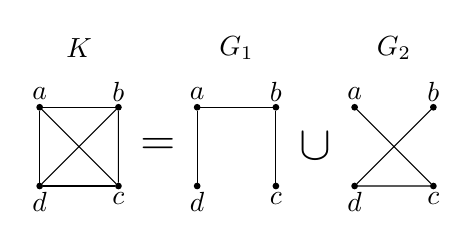
\begin{tikzpicture}[every node/.style={draw, circle, fill=black, minimum size=2pt, inner sep=0pt}]
          % First Graph
          \node (T)[draw=none, fill=none] at (0.5,0.75) {$K$};
          \node (0) at (0, 0)[label=above:$a$]  {};
          \node (1) at (1, 0)[label=above:$b$]  {};
          \node (2) at (1, -1)[label=below:$c$] {};
          \node (3) at (0, -1)[label=below:$d$] {};

          \draw (2) -- (3) -- (0) -- (1);
          \draw (0) -- (2) -- (1) -- (3);
          % "=" symbol
          \node[draw=none, fill=none] at (1.5, -0.5) {\LARGE $=$};

          % Second graph
          \begin{scope}[xshift=2cm]
            \node (T)[draw=none, fill=none] at (0.5,0.75) {$G_{1}$};
            \node (0) at (0, 0)[label=above:$a$]  {};
            \node (1) at (1, 0)[label=above:$b$]  {};
            \node (2) at (1, -1)[label=below:$c$] {};
            \node (3) at (0, -1)[label=below:$d$] {};

              \draw (3) -- (0) -- (1) -- (2);
          \end{scope}
          
          % "\cup" symbol
          \node[draw=none, fill=none] at (3.5, -0.5) {\LARGE $\cup$};
          
          \begin{scope}[xshift=4cm]
            \node (T)[draw=none, fill=none] at (0.5,0.75) {$G_{2}$};
            \node (0) at (0, 0)[label=above:$a$]  {};
            \node (1) at (1, 0)[label=above:$b$]  {};
            \node (2) at (1, -1)[label=below:$c$] {};
            \node (3) at (0, -1)[label=below:$d$] {};
              
            \draw (0) -- (2) -- (3) -- (1);
          \end{scope}
      \end{tikzpicture}
  \end{center}
  \caption{$\{G_{1},G_{2}\}$ is a $P_{3}$-decomposition of $K_{4}$ or a $P_{3}$-design of order $4$}
  \label{fig:Gdecompex}
\end{figure}
We know that if a $G$-decomposition of some graph $K$ exists, that all of it's members have the same number of edges and vertices. This allows us to find constraints on graphs $K$ that can be decomposed by some subgraph $G\subseteq K$ on $m$ edges solely based on divisiblity properties.

\begin{lemma}[Necessary Condition (general)] \label{lem:gencondition}
  Let $G$ be a simple graph on $m$ edges. There exists a $G$-decomposition of a graph $K$ only if $|E(G)|=m$ divides $|E(K)|$. 
\end{lemma}

  \begin{proof}
  Suppose there exists a $G$-decomposition $\{G_{1},\hdots, G_{n}\}$ of $K$. Then $E(G_{1})\sqcup \cdots \sqcup\,E(G_{t})=E(K)$ and so $|E(K)|=|E(G_{1})\sqcup \cdots \sqcup E(G_{t})|=|E(G_{1})|+ \cdots + |E(G_{t})|=tm$. So $|E(G)|=m$ divides $|E(K)|$.
  \end{proof}

\begin{thm}[Necessary Condition ($K_{n}$)] \label{thm:Kncondition}
  Let $G$ be a simple graph on $m$ edges. There exists a $G$-decomposition of $K_{n}$ only if $n$ is idempotent modulo $2m$; only if $n^{2}\equiv n\pmod{2m}$.
\end{thm}

\begin{proof}
  Suppose there exists a $G$-decomposition of $K_{n}$. Then $|E(G)|=m$ divides $|E(K_{n})|=\binom{n}{2}=\frac{n(n-1)}{2}$ by Lemma \ref{lem:gencondition}. Therefore, $\frac{n^{2}-n}{2}=mt$ for some $t\in \NN$. Observe.

  $$n^{2}-n= 2mt\implies n^{2}-n\equiv 0\pmod{2m}\implies n^{2}\equiv n\pmod{2m}.$$
\end{proof}
By the previous theorem, any graph on $m$ edges decomposes $K_{n}$ only if $n$ is idempotent modulo $2m$. Note that the converse isn't necessarily true. However, for a graph $G$ on $m$ edges, this finite set of constraints allows us to ask:
\begin{center}
For what $n$ is $K_{n}$ $G$-decomposable?
\end{center}
This question is known as the \textit{spectrum problem} for graph decompositions. Pioneering work by Rosa and Kotzig in the 1960s-especially in the development of graph labeling helped shape the modern approach to $G$-decomposition problems. Since then, labeling-based techniques and tools from design theory have driven significant progress. In particular, graph labeling methods have played a central role in addressing the spectrum problem for small graphs. This thesis project directly builds upon work by Freyberg and Peters, who recently solved the spectrum problem for forests with six edges~\cite{FreybergPeters2024}. Their paper provides a comprehensive summary of known decompositions for graphs $G$ with fewer than seven edges.

Using graph labelings to solve $G$-decomposition problems is basically about doing algebra on subgraphs in order to generate other edge-disjoint subgraphs while preserving isomorphism to $G$. If we take the vertices of a graph $K$ to be elements of a group, we can use the structure of the group to our advantage. Specifically, when $K\cong K_{n}$, and we take it's vertices to be $\ZZ_{n}$, and then we label the vertices of $G$ with some subset of $\ZZ_{n}$. There are various labeling techniques of this kind stemming from Rosa's work in the 1960s that that allow us permute or act on the labels of the vertices of $G$ with subgroups of $\ZZ_{n}$ to generate new isomorphic copies of $G$ which are pairwise edge-disjoint. In the next section, we provide a example which outlines in some detail how this machinery works for $G$-decompositions of complete graphs.
\section{Graph labelings}

Take the vertices of $K_{5}$ to be $\ZZ_{5}$ and arrange it in the same manner as in \ref{fig:K5}. Notice that every vertex shares an edge with two vertices directly adgacent to it and two vertices that are `two adjacencies away' on the outer cycle $(01234)$. We call this idea \textit{length} denoted $\ell$ where edges joining two vertices $u,v$ have length $\ell(uv)=l$ if they are `$l$ adjacencies away' from each other on the outer cycle. 

Formally, for $K_{n}$ we define the edge length function $\ell$ as follows:
$$\ell(uv)=\min\{|u-v|,n-|u-v|\}$$
Notice that for $K_{5}$, we only have lengths $1$ or $2$ as previously observed. Color the length $1$ edges \textcolor{blue}{blue}, and the length $2$ edges \textcolor{red}{red}. This is depicted in the figure below.

\begin{figure}[H]
  \begin{center}
  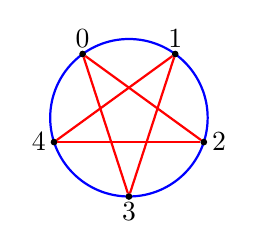
\begin{tikzpicture}[scale=1, every node/.style={draw, circle, fill=black, minimum size=2pt, inner sep=0pt}]
  
  % Outer circle in blue
  \draw[blue, thick] (0,0) circle (1);
  
  % Place nodes on the circle
  \node (0) at (126:1) [label=above:0]{};   % upper left
  \node (1) at (54:1)  [label=above:1]{};   % upper right
  \node (2) at (342:1) [label=right:2]{};   % lower right
  \node (3) at (270:1) [label=below:3]{};   % bottom
  \node (4) at (198:1) [label=left:4]{};   % lower left

  % Internal edges (diagonals) in red
  \draw[red, thick] (0) -- (2);
  \draw[red, thick] (1) -- (3);
  \draw[red, thick] (2) -- (4);
  \draw[red, thick] (3) -- (0);
  \draw[red, thick] (4) -- (1);
  
  \end{tikzpicture}
  \end{center}
  \caption{$K_{5}$ with lengths colored}
  \label{fig:K5colored}
\end{figure}
Now, consider $P_{3}$. It has $2$ edges, and $K_{5}$ has $\binom{5}{2}=10$ edges. Since $2|10$, by Lemma \ref{lem:gencondition} its \textit{possible} that a $P_{3}$-decomposition of $K_{5}$ exists. Now since $P_{3}$ has $2$ edges and there are $2$ lengths in $K_{5}$, what if we can just make sure each copy of $P_{3}$ has both a \textcolor{blue}{blue} edge and a \textcolor{red}{red} edge? How can we do that while ensuring that no edge is repeated?

It turns out that if we take the vertices of $K_{n}$ to be $\ZZ_{n}$, adding $1$ (and therefore anything) modulo $n$ to the endpoints of an edge preserves it's length. We call the act of permuting vertices in this manner (permuting by an element of the group) \textit{clicking} or \textit{developing}. If we are permuting all vertices of a labeling by the same group element, we often will just say we are developing the labeling by that group element.

In the context of our problem with $P_{3}$ and $K_{5}$, this means that if we label $P_{3}$ with elements of $\ZZ_{5}$ such that just have one \textcolor{blue}{blue} edge of length 1, and one \textcolor{red}{red} edge of length 2, that we can simply generate all edges of length $1$ and $2$ in $K_{n}$ (which is just all edges of $K_{n}$) while preserving the structure of the graph by developing our labeling by $1$. Label the defining path of $P_{3}$ via (2,0,1). Developing the vertices by $1$ (modulo $5$) will give all members of a $P_{3}$-decomposition of $K_{5}$. A decomposition that can generated by permuting all vertices of one labeling repeatedly in this fashion is called a \textit{cyclic decomposition}. This is depicted in the following figure.

\begin{figure}[H]
  \begin{center}
  \begin{tikzpicture}[scale=0.75, every node/.style={draw, circle, fill=black, minimum size=2pt, inner sep=0pt}]
  
  % Outer circle in blue
  %\draw[blue, thick] (0,0) circle (1);

  % (2,0,1)
  % Place nodes on the circle
  \node (0) at (126:1) [label=above:0]{};   % upper left
  \node (1) at (54:1)  [label=above:1]{};   % upper right
  \node (2) at (342:1) [label=right:2]{};   % lower right
  \node (3) at (270:1) [label=below:3]{};   % bottom
  \node (4) at (198:1) [label=left:4]{};   % lower left
      
  %Draw the outer cycle edges as arcs along the circle
  %\draw[blue, thick] (3) arc (270:342:1); %3 -- 2
  %\draw[blue, thick] (2) arc (342:414:1); %2 -- 1 
  \draw[blue, thick] (1) arc (54:126:1);  %1 -- 0
  %\draw[blue, thick] (0) arc (126:198:1); %0 -- 4
  %\draw[blue, thick] (4) arc (198:270:1); %4 -- 3

  % Internal edges (diagonals) in red
  \draw[red, thick] (0) -- (2);
  %\draw[red, thick] (1) -- (3);
  %\draw[red, thick] (2) -- (4);
  %\draw[red, thick] (3) -- (0);
  %\draw[red, thick] (4) -- (1);
  \node[draw=none, fill=none] at (1.75, 0) {\scriptsize $\overset{+1}{\longrightarrow}$};

  \begin{scope}[shift={(3.5,0)}]
    %(3,1,2)
    \node (0) at (126:1) [label=above:0]{};   % upper left
    \node (1) at (54:1)  [label=above:1]{};   % upper right
    \node (2) at (342:1) [label=right:2]{};   % lower right
    \node (3) at (270:1) [label=below:3]{};   % bottom
    \node (4) at (198:1) [label=left:4]{};   % lower left
        
    %Draw the outer cycle edges as arcs along the circle
    %\draw[blue, thick] (3) arc (270:342:1); %3 -- 2
    \draw[blue, thick] (2) arc (342:414:1); %2 -- 1 
    \draw[blue, dashed] (1) arc (54:126:1);  %1 -- 0
    %\draw[blue, thick] (0) arc (126:198:1); %0 -- 4
    %\draw[blue, thick] (4) arc (198:270:1); %4 -- 3

    % Internal edges (diagonals) in red
    \draw[red, dashed] (0) -- (2);
    \draw[red, thick] (1) -- (3);
    %\draw[red, thick] (2) -- (4);
    %\draw[red, thick] (3) -- (0);
    %\draw[red, thick] (4) -- (1);
    \node[draw=none, fill=none] at (1.75, 0) {\scriptsize $\overset{+1}{\longrightarrow}$};
  \end{scope}

  \begin{scope}[shift={(7,0)}]
    %(4,2,3)
    \node (0) at (126:1) [label=above:0]{};   % upper left
    \node (1) at (54:1)  [label=above:1]{};   % upper right
    \node (2) at (342:1) [label=right:2]{};   % lower right
    \node (3) at (270:1) [label=below:3]{};   % bottom
    \node (4) at (198:1) [label=left:4]{};   % lower left
        
    %Draw the outer cycle edges as arcs along the circle
    \draw[blue, thick] (3) arc (270:342:1); %3 -- 2
    \draw[blue, dashed] (2) arc (342:414:1); %2 -- 1 
    \draw[blue, dashed] (1) arc (54:126:1);  %1 -- 0
    %\draw[blue, thick] (0) arc (126:198:1); %0 -- 4
    %\draw[blue, thick] (4) arc (198:270:1); %4 -- 3

    % Internal edges (diagonals) in red
    \draw[red, dashed] (0) -- (2);
    \draw[red, dashed] (1) -- (3);
    \draw[red, thick] (2) -- (4);
    %\draw[red, thick] (3) -- (0);
    %\draw[red, thick] (4) -- (1);
    \node[draw=none, fill=none] at (1.75, 0) {\scriptsize $\overset{+1}{\longrightarrow}$};
  \end{scope}

  \begin{scope}[shift={(10.5,0)}]
    %(0,3,4)
    \node (0) at (126:1) [label=above:0]{};   % upper left
    \node (1) at (54:1)  [label=above:1]{};   % upper right
    \node (2) at (342:1) [label=right:2]{};   % lower right
    \node (3) at (270:1) [label=below:3]{};   % bottom
    \node (4) at (198:1) [label=left:4]{};   % lower left
        
    %Draw the outer cycle edges as arcs along the circle
    \draw[blue, dashed] (3) arc (270:342:1); %3 -- 2
    \draw[blue, dashed] (2) arc (342:414:1); %2 -- 1 
    \draw[blue, dashed] (1) arc (54:126:1);  %1 -- 0
    %\draw[blue, thick] (0) arc (126:198:1); %0 -- 4
    \draw[blue, thick] (4) arc (198:270:1); %4 -- 3

    % Internal edges (diagonals) in red
    \draw[red, dashed] (0) -- (2);
    \draw[red, dashed] (1) -- (3);
    \draw[red, dashed] (2) -- (4);
    \draw[red, thick] (3) -- (0);
    %\draw[red, thick] (4) -- (1);
    \node[draw=none, fill=none] at (1.75, 0) {\scriptsize $\overset{+1}{\longrightarrow}$};
  \end{scope}
  \begin{scope}[shift={(14,0)}]
    %(1,4,0)
    \node (0) at (126:1) [label=above:0]{};   % upper left
    \node (1) at (54:1)  [label=above:1]{};   % upper right
    \node (2) at (342:1) [label=right:2]{};   % lower right
    \node (3) at (270:1) [label=below:3]{};   % bottom
    \node (4) at (198:1) [label=left:4]{};   % lower left
        
    %Draw the outer cycle edges as arcs along the circle
    \draw[blue, dashed] (3) arc (270:342:1); %3 -- 2
    \draw[blue, dashed] (2) arc (342:414:1); %2 -- 1 
    \draw[blue, dashed] (1) arc (54:126:1);  %1 -- 0
    \draw[blue, thick] (0) arc (126:198:1); %0 -- 4
    \draw[blue, dashed] (4) arc (198:270:1); %4 -- 3

    % Internal edges (diagonals) in red
    \draw[red, dashed] (0) -- (2);
    \draw[red, dashed] (1) -- (3);
    \draw[red, dashed] (2) -- (4);
    \draw[red, dashed] (3) -- (0);
    \draw[red, thick] (4) -- (1);
  \end{scope}
  
  \end{tikzpicture}
  \end{center}
  \caption{A cyclic $P_{3}$-decomposition of $K_{5}$}
  \label{fig:P3K5colordecomp}
\end{figure}

Nice and easy right? But that's just one complete graph that $P_{3}$ can decompose. Remember, that it is \textit{possible} that $P_{3}$ can decompose any $K_{n}$ where $n\equiv n^{2} \pmod{4}$ by Theorem \ref{thm:Kncondition}. This equivalent to saying $n=4t+r$ where $r$ is an idempotent in the ring $\ZZ_{4}$ and $t\geq 1$. The idempotents in $\ZZ_{4}$ are $0,1$. So this means $\ZZ_{5}$ is just a special case of $n$ where $n=4t+1$ where $t=1$. Luckily, even though these are infinite families, it is known that for each step $t\mapsto t+1$, new lengths come $2$ at a time. This means if we can somehow transform our labeling at each step to include the new lengths, we can maybe take care of the entire family $K_{4t+1}$. We want to fine tune our labeling to be able to weather this process. This is what graph labeling is all about. Note that if $r$ was not $0$ or $1$, we would need multiple labelings to take care of the whole family. This is explained later in this paper.

Lastly, some basic observations about a general subgraph $G\subseteq K_{n}$ with $m$ edges of $K_{n}$. The maximal length in $K_{n}$ is $\floor{\frac{n}{2}}$. This is intuitive, since when you travel halfway across the outer cycle from some vertex, the lengths start going back down again as you begin nearing that vertex again. Now, $n$ must be of the form $2mt+r$ where $t\geq 1$ and $r$ is an idempotent in the ring $\ZZ_{2m}$. This means that in $K_{2m+r}$ if $\ell(uv)=|u-v|<\floor{\frac{2m+r}{2}}<\floor{\frac{2mt+r}{2}}$ for $t>1$, then $\ell(uv)=|u-v|$ in all $K_{2mt+r}$ for $t\geq 1$. this is important, because at each step $t\mapsto t+1$, new lengths come $m$ at a time.

Now, for $r=0$ or $1$, if a certain labeling of a graph $G$ on $m$ edges exists, there exists a $G$-decomposition of $K_{2mt+r}$ for $t\geq 1$. However, if $r\neq 0,1$, one labeling will not suffice and other techniques are needed to prove that $G$ decomposes $K_{2mt+r}$ for $t\geq 1$. These labelings and techniques are defined as they are needed in the proceeding chapters. Finally, we are ready to introduce the focus of this project.
\section{Seven edge forests}
This project continues on Freyberg and Peters' work on six edge forests by asking the same question about seven edge forests:
\begin{center}
  Let $F$ be a forest on seven edges. For which $n$ does $F$ decompose $K_{n}$? 
\end{center}
The spectrum problem for the matching $\mathbf{7T_{2}^{11}}$ was solved by de Werra in $1970$. Every component of a forest on seven edges is a tree on six or less edges which are cataloged in Figure \ref{fig:catalog}. We use the naming convention $\mathbf{T_{j}^i}$ to denote the $i^{\textrm{th}}$ tree with $j$ vertices and we index the vertices $v_{1}$ through $v_{j}$ for each tree as specified below.

\begin{figure}[H]
\begin{center}
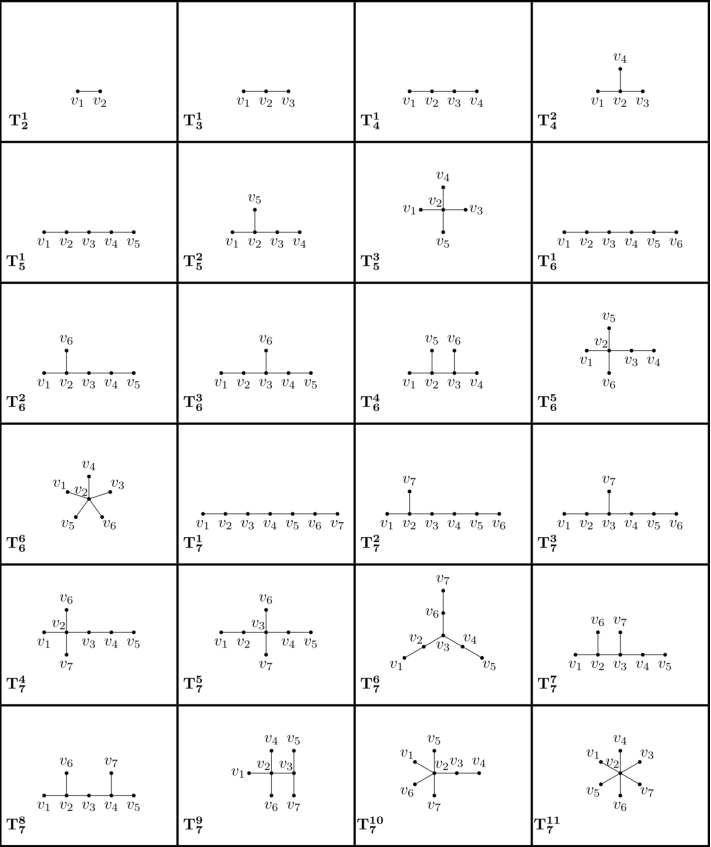
\includegraphics[scale=0.85]{standalone/tree-chart}
\end{center}
\caption{Trees with less than seven edges}
\label{fig:catalog}
\end{figure}

The next theorem gives the necessary conditions for the existence of a $G$-decomposition of $K_n$ when $G$ is a graph with 7 edges.

\begin{thm}\label{thm:forestcondition}

  If $G$ is a graph with $7$ edges and a $G$-decomposition of $K_n$ exists, then $n \equiv 0,1,7, \textrm{or} \; 8 \pmod{14}$.

\end{thm}
\begin{proof}
    If a $G$-decomposition of $K_{n}$ exists, then $n$ is idempotent modulo $2(7)=14$ by Theorem \ref{thm:Kncondition} which immediately implies that $n \equiv 0,1,7, \textrm{or} \; 8 \pmod{14}$ since those are all the idempotents in $\ZZ_{14}$.
\end{proof}

For this project, we do not define the graph on one vertex to be a tree. This means that any connected component in a forest has at least one edge and we also require there to be at least two connected components. There are $47$ such forests with $7$ edges up to isomorphism.  As stated previously, the matching on seven edges is solved, so only the remaining $46$ trees need be considered in the subsequent chapters. Chapter \ref{chap:0,1(mod 14)} handles decomposing $K_{n}$ into all $47$ forests when $n \equiv 0 \textrm{ or } 1 \pmod{14}$. Chapter \ref{chap:7,8 (mod 14)} applies to all the forests when $n \equiv 7 \textrm{ or } 8 \pmod{14}$ with the lone exception of $\mathbf{T_{7}^{11}}\sqcup\mathbf{T_{2}^{1}},$ which is solved for those values of $n$ in Chapter \ref{chap:special case}.

After proving the main result of this project, we provide a couple of additional results in Chapter \ref{chap:Additional Results}: (1) An edge mapping that depends on $t$ and preserves lengths for wraparound edges in $K_{3m}$ and $K_{3m+1}$ to $K_{2mt+m}$ and $K_{2mt+m+1}$, respectively, for each step $t\mapsto t+1$. (2) Galaxy decompositions of complete bipartite graphs. This chapter concludes the main results of this thesis project.

We then present some \verb|python| programs in Chapter \ref{chap:programming} that were created as a result of this thesis project. One is \verb|tikzgrapher|: A new graph visualization program, which was built from scratch only using \verb|Pygame| and \verb|NetworkX| and several other basic libraries. It allows one to visualize simple \verb|NetworkX| graphs in an interactive \verb|Pygame| window that allows for colorings and custom labelings along with dragging and moving components of the graph. A main feature\ is that the user can save the graph layout depicted in the \verb|Pygame| window as a \verb|Tik| graph in a standalone \LaTeX$\,$file. \verb|tikzgrapher| is paired with a graph labeling solver. This is a constraint programming project that can find several labelings on graphs if they exist. The Conclusion follows this chapter, then a list of References and an Appendix of labelings marks the end of the paper.




%\begin{itemize}

%\item Chapter 1 introduces the analytic goals pursued in this thesis.

%\item Chapter 2 briefly presents the history of, and science behind, the
%subjects presented in this thesis.

%\item In Chapter 3 the experiment is outlined.

%\item Chapter 4 describes the simulation process used in the analysis.

%\item Chapter 5 follows the chain of reconstruction software used to obtain
%meaningful results from data.

%\item Chapter 6 hashes out the strategy for analysis and presents the data and
%simulated sets that will be used in the analysis.

%\item Chapter 7 demonstrates the implementation of the event selection
%processes.

%\item In Chapter 8 those events selected in Chapter 7 are analyzed.

%\item Chapter 9 presents a final discussion of the analyses presented in the
%thesis.

%\end{itemize}
%%%%%%%%%%%%%%%%%%%%%%%%%%%%%%%%%%%%%%%%%%%%%%%%%%%%%%%%%%%%%%%%%%%%%%%%%%%%%%%%
